%
% $Id: ch03_thework.tex
%
%   *******************************************************************
%   * SEE THE MAIN FILE "AllegThesis.tex" FOR MORE INFORMATION.       *
%   *******************************************************************
%
\chapter{Method of Approach} \label{ch:methods}

\name\ was developed using a modified agile approach; short development ``sprints'' were executed for key system development.
We describe the product of some of those sprints in Section~\ref{ch:methods:renderer}, primarily the ray-tracing engines.
In Section~\ref{ch:methods:interface} we also describe the Tickit interface and its algorithms.
Finally, in Section~\ref{ch:methods:threats}, we discuss drawbacks, challenges, and failures in development, as well as directions for future improvement as an open source project.


\section{Renderer Implementation} \label{ch:methods:renderer}
While building \name, two separate render engine prototypes were implemented.
The first, which we describe in Section~\ref{ch:methods:renderer:sequential}, was a simple, single core sequential renderer \cite{raytermCpuImpl}.
This engine was developed in three main development sprints, over a period of about two months.
The second, described in Section~\ref{ch:methods:renderer:parallel}, uses CUDA \cite{nvidia2011cuda} and OptiX \cite{parker2010optix} to leverage GPU compute power in parallel.
This engine was developed over two sprints, in a little under a month.


\subsection{Sequential} \label{ch:methods:renderer:sequential}

The sequential renderer, or as its implementation calls it, \texttt{rayterm-cpu}, is a CPU-only ray-tracer.
It supports three different types of materials: diffuse, metallic, and dielectric.
These materials are complemented with two geometric primitives: disks, and spheres.
Figure~\ref{fig:rayterm-cpu-ppm} shows an image of the \texttt{ppm} output of \texttt{rayterm-cpu} near the end of its development.
The Tickit interface was never integrated into the CPU implementation, as this implementation is not performant enough for even simple scenes at low resolution.
For example, Figure~\ref{fig:rayterm-cpu-ppm} was rendered in about 20 seconds on a modern CPU.

\begin{figure}[htb]
  \centering
  \includegraphics[width=0.75\textwidth]{impl-images/first_positionable_camera}
  \caption{\texttt{rayterm-cpu} example \texttt{ppm} output}
  \label{fig:rayterm-cpu-ppm}
\end{figure}

The main advantage of a sequential renderer is the lower development overhead, since there is no need to interface with a complex device such as a GPU.
This means that there is no need for handling parallel execution, and each ray is computed one after the other.
Because of this simplicity, this engine's development was perfectly suited the goal of gaining knowledge  and experience in ray-tracing.
The development also explored many fundamentals so that future contributions would be well-founded.
With 219 commits and over a thousand lines of code in the final product, along with many thousands of additions and deletions, \texttt{rayterm-cpu} accomplished its goals.

\littlesection{Components} \label{ch:methods:renderer:sequential:components}

The sequential renderer's implementation relies on two main components, as well as the Eigen linear algebra library \cite{eigenweb}.
These components have a linear relationship, as can be seen in Figure~\ref{fig:rayterm-cpu-components}; \texttt{raytrace} deals with tracing rays, \texttt{raymath} with intersection logic, and Eigen with linear algebra.

\begin{figure}[htb]
  \centering
  \begin{subfigure}[htb]{0.4\textwidth}
  \hspace{0.25\textwidth}
  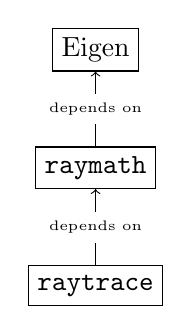
\begin{tikzpicture}
      \node[shape=rectangle,draw=black] (e) at (0,1.5) {Eigen};
      \node[shape=rectangle,draw=black] (rm) at (0,0) {\texttt{raymath}};
      \node[shape=rectangle,draw=black] (rt) at (0,-1.5) {\texttt{raytrace}};

      \path [<-](e) edge node[midway, fill=white] {\tiny depends on} (rm);
      \path [<-](rm) edge node[midway, fill=white] {\tiny depends on} (rt);
  \end{tikzpicture}
  \caption{Component and dependency relationships in \texttt{rayterm-cpu}}
  \label{fig:rayterm-cpu-components}
  \end{subfigure}
  \begin{subfigure}[htb]{0.4\textwidth}
    \hspace{0.25\textwidth}
    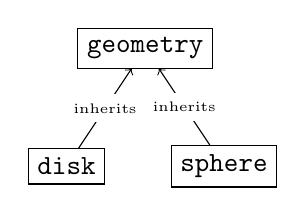
\begin{tikzpicture}
      \node[shape=rectangle,draw=black] (g) at (0,1.5) {\texttt{geometry}};
        \node[shape=rectangle,draw=black] (s) at (1,0) {\texttt{sphere}};
        \node[shape=rectangle,draw=black] (d) at (-1,0) {\texttt{disk}};

        \path [<-](g) edge node[midway, fill=white] {\tiny inherits} (s);
        \path [<-](g) edge node[midway, fill=white] {\tiny inherits} (d);
    \end{tikzpicture}
    \caption{Geometric structures in \texttt{raymath}}
    \label{fig:rayterm-cpu-raymath}
  \end{subfigure}
  % \caption{}
  \label{fig:rayterm-cpu-first-diagrams}
\end{figure}



\littlesection{Design} \label{ch:methods:renderer:sequential:design}

This section is about the code structure and organization in the \texttt{rayterm-cpu} implementation.

\begin{enumerate}
  \item geometry defs
  \item material defs
  \item world defs
  \item renderer structure
\end{enumerate}

\littlesection{Algorithms} \label{ch:methods:renderer:sequential:algorithms}

This is a demonstration section on what the current cpu implementation is capable of; images and the like will be included.

\littlesection{Prototype} \label{ch:methods:renderer:sequential:prototype}

This section describes the lessons learned from CPU implementation, and how the GPU implementation will differ and improve because of this step.
It will also briefly reflect on challenges, and reference Section~\ref{ch:methods:threats}.

\subsection{Parallel} \label{ch:methods:renderer:parallel}

Introduction to parallel GPU renderer, description of parallel, short GPU intro (reference introduction).

With 227 commits and over 1.5 thousand lines of code in the renderer alone, along with many thousands of additions and deletions, \texttt{rayterm} has a good start on its life.
There are many, many more improvements possible, however.
We detail some of them in the context of the larger \name\ implementation in Section~\ref{ch:methods:threats}.

\littlesection{Libraries} \label{ch:methods:renderer:parallel:libraries}

This section talks about OptiX and CUDA.

\littlesection{Design} \label{ch:methods:renderer:parallel:design}

This section is about the code structure and organization in the \texttt{rayterm} implementation.

\littlesection{Demonstration} \label{ch:methods:renderer:parallel:demo}

This is a demonstration section on final renderer is capabable of -- this section uses only \texttt{ppm} output.

\section{Interface Implementation} \label{ch:methods:interface}

\subsection{Design} \label{ch:methods:interface:design}

\section{Threats and the Future} \label{ch:methods:threats}

CPU:
\begin{enumerate}
  \item metal bug
  \item blender comparisons
  \item space differential
  \item coordinate systems
  \item research difficulty (can't read a physics textbook for each material)
\end{enumerate}

GPU:
\begin{enumerate}
  \item Travis testing
  \item library management
  \item gradle integration
  \item [...]
\end{enumerate}
